\chapter{Исследовательская часть}
\section{Технические характеристики}
Тестирование выполнялось на устройстве со следующими техническими характеристиками:
\begin{itemize}
	\item Операционная система Pop!\_OS 22.04 LTS \cite{ubuntu} Linux \cite{linux};
	\item Оперативная память 16 Гб;
	\item Процессор AMD® Ryzen 7 2700 eight-core processor × 16 \cite{amd}.
\end{itemize}
Во время тестирования устройство было подключено к блоку питания и не нагружено никакими приложениями, кроме встроенных приложений окружения, окружением и системой тестирования.

\section{Демонстрация работы программы}



На рисунке \ref{demonstration} представлен результат работы программы.

\begin{figure}[ht!]
	\begin{center}
		\captionsetup{singlelinecheck = false, justification=centerfirst}
		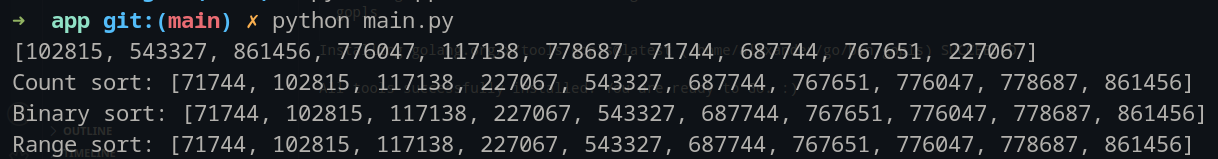
\includegraphics[scale=0.8]{assets/demonstation.png}
		\caption{Пример работы программы}
		\label{demonstration}
	\end{center}
	
	
\end{figure}

\newpage

\section{Время выполнения алгоритмов}

Результаты замеров времени работы реализаций алгоритмов сортировки на различных входных данных (в мс) приведены в таблицах \ref{tbl:best}, \ref{tbl:worth} и \ref{tbl:random}.

\begin{table}[ht!]
	\begin{center}
			\captionsetup{justification=raggedleft,singlelinecheck=off}
			\caption{Результаты замеров реализаций сортировок, входными данными явллялись отсортированные по возрастанию значений массивы.}
			\label{tbl:best}
			\begin{tabular}{|c|c|c|c|}
				\hline
				Размер & Подсчетом &  Поразрядная &  Бинарным деревом \\
				\hline
				100 & 0.1662 & 0.0714 & 0.8650 \\ 
				\hline
				200 & 0.5113 & 0.2058 & 3.3357 \\ 
				\hline
				300 & 1.1026 & 0.3131 & 7.6464 \\ 
				\hline
				400 & 2.0140 & 0.4364 & 13.6841 \\ 
				\hline
				500 & 3.3046 & 0.5591 & 21.5524 \\ 
				\hline
				600 & 5.0567 & 0.6798 & 31.3052 \\ 
				\hline
				700 & 6.6944 & 0.7852 & 43.0406 \\ 
				\hline
				800 & 8.5163 & 0.8766 & 56.4318 \\ 
				\hline
			\end{tabular}
	\end{center}
\end{table}


\begin{table}[ht!]
	\begin{center}
			\captionsetup{justification=raggedleft,singlelinecheck=off}
			\caption{Результаты замеров реализаций сортировок, входными данными явллялись отсортированные по убыванию значений массивы.}
			\label{tbl:worth}
			\begin{tabular}{|c|c|c|c|}
				\hline
				Размер & Подсчетом &  Поразрядная &  Бинарным деревом \\
				\hline
				100 & 0.1606 & 0.1048 & 0.7138 \\ 
				\hline
				200 & 0.5005 & 0.2008 & 2.7633 \\ 
				\hline
				300 & 1.0747 & 0.3110 & 6.3060 \\ 
				\hline
				400 & 1.9383 & 0.4312 & 11.3831 \\ 
				\hline
				500 & 3.1148 & 0.5427 & 18.0577 \\ 
				\hline
				600 & 4.6409 & 0.6693 & 26.0260 \\ 
				\hline
				700 & 6.7969 & 0.8317 & 36.7397 \\ 
				\hline
				800 & 8.7922 & 0.9583 & 47.2628 \\ 
				\hline
			\end{tabular}
	\end{center}
\end{table}

\newpage

\begin{table}[ht!]
	\begin{center}
			\captionsetup{justification=raggedleft,singlelinecheck=off}
			\caption{Результаты замеров реализаций сортировок, входными данными явллялись заполненные числами со случайными значениями массивы.}
			\label{tbl:random}
			\begin{tabular}{|c|c|c|c|}
				\hline
				Размер & Подсчетом &  Поразрядная &  Бинарным деревом \\
				\hline
				100 & 0.2734 & 0.1043 & 0.1560 \\ 
				\hline
				200 & 0.8321 & 0.2090 & 0.3756 \\ 
				\hline
				300 & 1.6837 & 0.3142 & 0.6025 \\ 
				\hline
				400 & 2.8938 & 0.4281 & 0.9785 \\ 
				\hline
				500 & 4.4438 & 0.5419 & 1.1784 \\ 
				\hline
				600 & 6.4153 & 0.6704 & 1.5523 \\ 
				\hline
				700 & 8.6692 & 0.7678 & 1.9018 \\ 
				\hline
				800 & 11.3752 & 0.8992 & 2.2986 \\ 
				\hline
			\end{tabular}
	\end{center}
\end{table}

\newpage
\section{Графики функций}


	\begin{figure}[b]{\textwidth}
		\centering
		\begin{tikzpicture}
			\begin{axis}[
				xlabel={размер массива},
				ylabel={время, ns},
				width = 0.95\textwidth,
				height=0.3\textheight,
				xmin=0, xmax=1000,
				legend pos=north west,
				xmajorgrids=true,
				grid style=dashed,
				]
				\addplot[
				blue,
				semithick,
				mark = x,
				mark size = 3pt,
				thick,
				] file {assets/count_r.dat};
				
				\addplot[
				red,
				semithick,
				mark = *,
				] file {assets/count_r.dat};
				
				\addplot[
				green,
				semithick,
				mark = *,
				] file {assets/count_r.dat};
				
				\legend{
					Сортировка подсчетом,
					Сортировка поразрядная,
					Сортировка бинарным деревом,
				}
			\end{axis}
		\end{tikzpicture}
		\caption{Результаты замеров реализаций сортировок, входными данными явллялись заполненные числами со случайными значениями массивы.}
	\end{figure}
	\hfill
	\newline
	\begin{figure}[b]{\textwidth}
	\centering
	\begin{tikzpicture}
		\begin{axis}[
			xlabel={размер массива},
			ylabel={время, ns},
			width = 0.95\textwidth,
			height=0.3\textheight,
			xmin=0, xmax=1000,
			legend pos=north west,
			xmajorgrids=true,
			grid style=dashed,
			]
			\addplot[
			blue,
			semithick,
			mark = x,
			mark size = 3pt,
			thick,
			] file {assets/count_r.dat};
			
			\addplot[
			red,
			semithick,
			mark = *,
			] file {assets/count_r.dat};
			
			\addplot[
			green,
			semithick,
			mark = *,
			] file {assets/count_r.dat};
			
			\legend{
				Сортировка подсчетом,
				Сортировка поразрядная,
				Сортировка бинарным деревом,
			}
		\end{axis}
	\end{tikzpicture}
	\caption{Результаты замеров реализаций сортировок, входными данными явллялись заполненные числами со случайными значениями массивы.}
\end{figure}
	\begin{figure}[b]{\textwidth}
	\centering
	\begin{tikzpicture}
		\begin{axis}[
			xlabel={размер массива},
			ylabel={время, ns},
			width = 0.95\textwidth,
			height=0.3\textheight,
			xmin=0, xmax=1000,
			legend pos=north west,
			xmajorgrids=true,
			grid style=dashed,
			]
			\addplot[
			blue,
			semithick,
			mark = x,
			mark size = 3pt,
			thick,
			] file {assets/count_r.dat};
			
			\addplot[
			red,
			semithick,
			mark = *,
			] file {assets/count_r.dat};
			
			\addplot[
			green,
			semithick,
			mark = *,
			] file {assets/count_r.dat};
			
			\legend{
				Сортировка подсчетом,
				Сортировка поразрядная,
				Сортировка бинарным деревом,
			}
		\end{axis}
	\end{tikzpicture}
	\caption{Результаты замеров реализаций сортировок, входными данными явллялись заполненные числами со случайными значениями массивы.}
\end{figure}
\hfill
\hfill
	\hfill
	
\end{figure}

\newpage

\section*{Вывод}

В данном разделе были сравнены алгоритмы по времени.
Оптимизированный алгоритм Винограда является самым быстрым, за счет проведенных изменений в стандартном алгоритме Винограда.
